\documentclass[oneside]{ZJUthesis}
% 该文档中首字符为“%”的均为注释行,不会在论文中出现

% 论文默认为单面模式,需单面模式请将第一行换为如下所示:
%\documentclass[twoside]{ZJUthesis}

\input{ctex-xecjk-winfonts.def}
\usepackage{tikz-network}
\usepackage{bussproofs}
\usepackage{listings}
\usepackage{tikz}
\allowdisplaybreaks
%\usepackage[mathscr]{euscript}
%\let\euscr\mathscr \let\mathscr\relax% just so we can load this and rsfs
\usepackage{amssymb}
\let\oldemptyset\emptyset
\let\emptyset\varnothing
\newcommand{\powerset}{\raisebox{.05\baselineskip}{\Large\ensuremath{\wp}}}
\newcommand{\lamst}[0]{\ensuremath{\lambda{\rightarrow}}}
\newcommand{\HOL}[0]{\ensuremath{\mathrm{HOL}}}
\newcommand{\aml}[0]{\ensuremath{\mathrm{A}^{\lamst}}}
\newcommand{\amlh}[0]{\ensuremath{\mathrm{A}_{\HOL}^{\lamst}}}
\newcommand{\amlhF}[0]{\ensuremath{\mathrm{\d{A}}_{\HOL}^{\lamst}}}
\newcommand{\amlhC}[0]{\ensuremath{\dot{\mathrm{A}}_{\HOL}^{\lamst}}}
\newcommand{\amlN}[0]{\ensuremath{\mathrm{A}_0^{\lamst}}}
\newcommand{\amlhWASM}[0]{\ensuremath{\mathrm{A}_{\HOL}^{\lamst}{-}\mathrm{WASM}}}
\newcommand{\mbar}[0]{\ensuremath{\ |\ }}
\newcommand{\phety}[0]{\ensuremath{\mathrm{ph}}}
\newcommand{\natn}[0]{\ensuremath{\mathrm{number}}}
\newcommand{\bnf}[1]{\ensuremath{\langle\ #1\ \rangle}}
\newcommand{\itp}[1]{\ensuremath{#1\ \mathrm{interpretation}}}
\newcommand{\phenomenon}{\ensuremath{\mathrm{phenomenon}}}
\newcommand{\widesqa}[2][1.5]{
  \mathrel{\overset{#2}{\scalebox{#1}[1]{$\rightsquigarrow$}}}
}
\newcommand{\widesim}[2][1.5]{
  \mathrel{\overset{#2}{\scalebox{#1}[1]{$\sim$}}}
}
\newcommand{\widesims}[3][1.5]{
  \mathrel{\underset{#3}{\overset{#2}{\scalebox{#1}[1]{$\sim$}}}}
}
\renewcommand{\qedsymbol}{$\blacksquare$}
\newcommand{\proctr}[1]{\ensuremath{\prec #1 \succ}}



% 取消目录中链接的颜色,方便打印
% 如需颜色,请将“false”改为“true”
\hypersetup{colorlinks=false}

\begin{document}
	%%%%%%%%%%%%%%%%%%%%%%%%%%%%%
	%% 正文字体设定
	%%%%%%%%%%%%%%%%%%%%%%%%%%%%%
	\songti
	
	%%%%%%%%%%%%%%%%%%%%%%%%%%%%%
	%% 论文封面部分
	%%%%%%%%%%%%%%%%%%%%%%%%%%%%%
	% 中文封面内容
	
	% 中图分类号
	\classification{TP391}
	
	% 单位代码
	\serialnumber{10335}
	
	% 密级,如需密级则将其前“%”去掉
	%\SecretLevel{}
	
	% 学号
	\PersonalID{21721306}
	
	\title[]{基于经典逻辑上抽象机器的形式化方法}
	% 如果标题一行写不下,就写成两行,在下面的命令里写第二行,不需要两行则注释掉
    %\titletl{第二行}
	
	%英文题目
	\Etitle{A formal method via abstract machine}
	% 如果一行写不下,同中文题目设定,一行写不下则写两行,不需要就注释掉
	\Etitletl{on classical logic}
	%\Etitletll{An Oriental View}s
	
	% 作者
	\author{徐启源}
	\Eauthor{Qiyuan Xu}
	
	\degree{硕士}
	\Edegree{Master of Engineering}
	
	% 导师
	\supervisor{张\ \ 三\ \ 教授} \Esupervisor{Prof. San Zhang}
	
	% 合作导师,如果有的话,去掉注释,
	\cpsupervisor{刘长发\ \ 教授}
	\Ecpsupervisor{Prof. Changfa Liu}
	
	% 专业名称
	\major{计算机应用技术} \Emajor{Computer Application Technology}
	
	% 研究方向
	\researchdm{形式化方法} \Eresearchdm{Formal Method}
	
	% 所属学院
	\institute{计算机科学与技术学院} \Einstitute{College of Computer Science and Techonology}
	
	% 答辨日期
	%\defenddate{2011年11月1日}
	
	% 生成封面
	\makeCoverPage
	
	% 生成英文封面
	\makeECoverPage
	
	%%%%%%%%%%%%%%%%%%%%%%%%%%%%%%
	%% 原创声明与版权协议页
	%%%%%%%%%%%%%%%%%%%%%%%%%%%%%%
	
	% 生成原创声明与版权协议页
	%\makeOSandCPRTpage
	
	
	%%%%%%%%%%%%%%%%%%%%%%%%%%%%%%
	%% 论文部分开始
	%%%%%%%%%%%%%%%%%%%%%%%%%%%%%%
	\ZJUfrontmatter
	
	%%%%%%%%%%%%%%%%%%%%%%%%%%%%%%
	%% 摘要
	%%%%%%%%%%%%%%%%%%%%%%%%%%%%%%
	\begin{abstract}
\pagenumbering{roman}

%软件的正确性由其设计的正确性与其程序实现的正确性组成。
%软件设计的正确与否也许是难以评判的。
%而对程序实现正确性验证的探索,围绕着形式化方法特别是其中的形式化验证,
%自计算机科学伊始的1940年代就开始了。
%近百年过去了,大量的成果涌现,已经有很多方法能够证明程序实现的正确性,
%并构造这些正确性被证明的程序实现。
%然而,因为实践上的困难,特别是对于复杂软件过于高昂的证明成本,
%这些方法并未普遍地用于普通软件工业领域。
%程序实现上的缺陷始终存在,且一直在造成各种严重的损失。
%本文提出一种新的形式方法,试图完整地证明程序实现的正确性,并保持合理的成本。

本文首先提出一种新的公理系统,Noesis 系统,描述程序与其抽象语义(Abstract
 Semantic)的关联,以允许证明抽象语义的性质来证明程序的性质,
于是对程序的形式化验证转化为对抽象语义的验证,形式化验证就被简化。
然后本文围绕 Noesis 系统提出一种技术,通过演绎 Noesis 定理构造具有明确抽象语义的
程序。如此构造的程序具有良好的执行性能,并且对其的分析转变为更容易的,
对其抽象语义的分析,进而易于形式化验证,并可以利用已有的交互式定理证明工具最终
完成对其的形式化验证。
最终本文设计并实现了工具 \Eamlh 以实现该技术,并完成了编译到智能合约平台 EOS.IO 的编译后端,
可以生产高执行效率的并且易于形式化分析的智能合约。

指令集、常量集跟它们的抽象语义是 Noesis 系统的公理;
Noesis 系统上的定理表达,由这些
指令与常量组合而成的某个程序在此公理下所具有的抽象语义。
当作为公理的指令与常量的抽象语义正确地映射到某个执行环境时,
Noesis 系统上的定理即正确反映此执行环境上的程序的抽象语义。
若指令与常量存在到某个执行环境的机器代码的映射,则 Noesis 系统上的程序
可以编译到此执行环境。

Noesis 系统可以实现在经典逻辑上或者说作为经典逻辑的子集,
在本文中它被实现在 HOL 定理证明器的 HOL 逻辑上,
程序的抽象语义被自然地表达为 HOL 证明器上的数学对象,
可以使用 HOL 证明器分析与证明抽象语义的性质。
于是对程序的形式化验证变为对其抽象语义的形式化验证,而抽象语义是易于
分析的,于是形式化验证就被有效简化。


\keywords{公理系统,形式化验证,类型系统,智能合约,程序语义}
\end{abstract}

	
	%%%%%%%%%%%%%%%%%%%%%%%%%%%%%%
	%% 英文摘要
	%%%%%%%%%%%%%%%%%%%%%%%%%%%%%%
	\begin{englishabstract}

Correctness of software consists of correctness of the design and correctness of the
implementation.
While correctness of design maybe hard to judge, attemption for proof of the implementation 
correctness has begun from 1940s, focusing on formal method and formal verification especially.
Almost one hundred years past, with a great lot of achievements and numerous ways to 
prove the implementation correctness, 

软件的正确性由其设计的正确性与其程序实现的正确性组成。
软件设计的正确与否也许是难以评判的。
而对程序实现正确性验证的探索,围绕着形式化方法特别是其中的形式化验证,
自计算机科学伊始的1940年代就开始了。
近百年过去了,大量的成果涌现,已经有很多方法能够证明程序实现的正确性,
并构造这些正确性被证明的程序。
然而,因为实践上的困难,特别是对于复杂软件过于高昂的证明成本,
这些方法并未普遍地用于普通软件工业领域。
程序实现上的缺陷始终存在,且一直在造成各种严重的损失。
本文提出一种新的形式方法,试图完整地证明程序实现的正确性,并保持合理的成本。

著名的 Curry-Howard 同构揭示了程序与证明之间的内在联系,定理的演绎对应于程序的构建。
本文的思想基于此,
    \begin{center} \it 演绎定理以构建程序。 \end{center}
本文先提出了一种类型关系的扩广——Noesis 对应,一种三元关系将程序与不同理解下的抽象意义
联系起来,围绕此构建的形式系统成为类型系统的扩广。进而可以在一个成熟的定理证明器
上演绎 Noesis 对应关系的定理,以构建程序,并在定理证明器的保障下得到程序的抽象意义对应。
且此抽象意义是数学友好的数学对象,易于形式分析与证明。
于是对程序性质的证明可以转化为对数学友好的抽象意义的证明,进而有效简化了形式化验证。
且若在定理证明器上以该定理证明器的形式语言同样抽象地描述程序的设计,就可以
证明程序的抽象意义与程序设计的相等性,进而彻底而严谨地证明程序实现对此设计的正确性。
  最后本文以智能合约为应用场景实验性地实现了此方案,作为对其可行性的证明。
	
	\englishkeywords{1, 2, 3, 4}

\end{englishabstract}

	
	%%%%%%%%%%%%%%%%%%%%%%%%%%%%%%
	%% 目录页
	%%%%%%%%%%%%%%%%%%%%%%%%%%%%%%
	\ZJUcontents
	
	%%%%%%%%%%%%%%%%%%%%%%%%%%%%%%
	%% 插图列表
	%%%%%%%%%%%%%%%%%%%%%%%%%%%%%%
	\ZJUListofFigures
	
	%%%%%%%%%%%%%%%%%%%%%%%%%%%%%%
	%% 表格列表
	%%%%%%%%%%%%%%%%%%%%%%%%%%%%%%
	\ZJUListofTables
	
	
	%%%%%%%%%%%%%%%%%%%%%%%%%%%%%%
	%% 正文内容部分开始
	%%%%%%%%%%%%%%%%%%%%%%%%%%%%%%
	\ZJUmainmatter
	
	\chapter{绪论} \label{Ch.intro}
\section{研究背景与意义}

软件开发的主要挑战是在有限而可控的的时间与经费预算下开发高质量的软件
\cite{DinesSE1, brooks1995mythical}。
大量的方法提出以提升软件工程的效率与产品的质量
\cite{DinesSE1, SoftwareQuality}。
形式化方法(formal method)也可有效地应用于此,
以提升软件质量,并辅助软件的开发以提升开发效率\cite{formal_method_view1} 。
实际上大量的形式化方法已经在实际地发挥作用\cite{pierce2002types, jackson2012software}。

其中重要的一点是程序实现的验证,即一实现是否正确实现了设计的全部功能,且
不具有违背设计的包括漏洞在内的任何缺陷。
传统的单元测试难以发掘程序的全部潜在缺陷,
而相比而言形式化验证可以更有效地验证程序实现而发现更多的缺陷
\cite{formal_method_view1}。
但问题在于,倘若某种可行的形式化验证仅仅是更有效而并非是彻底,
即被验证后的程序实现依旧可能存在种种缺陷,
那这种形式化验证只能称之为比传统测试更好,
但问题仍未被彻底解决,仍然不能说一个实现是对于设计正确的满足而无任何缺陷。

软件的正确性包括其设计的正确性与程序实现的正确性。
软件的设计可能有缺陷,也许难以预见而难以检验,
但是否有可能一个程序的实现是彻底正确而无缺陷地满足了其设计?
进而能否验证一个程序是否被正确实现?
再而能否构造正确实现的而无任何缺陷的程序,
即所谓被验证的程序(verified software)\cite{verified_soft_grand}?

这一点具有实际的意义。
特别是在安全严苛(Safety critical)\cite{DinesSE1}的场景上尤其紧要。
有太多的计算机硬件与软件系统直接与生命安全、重要的民生事务相关。

本工作聚焦的基于区块链技术的各种智能合约平台就是这样的安全严苛场景。
因为区块链技术与平台的特殊性,被叫做智能合约的程序一旦被部署往往就无法修改,
进而无法更新以修复任何部署前未被发现的缺陷 \cite{swan2015blockchain}。
而目前区块链技术与智能合约平台大量应用于金融领域,如 Bitcoin 等诸多的
加密货币\cite{narayanan2016bitcoin},与加密金融这一新领域\cite{came2019}。
短短的数年以来智能合约领域已有大量的缺陷案例\cite{atzei2016survey}。
这些缺陷往往会导致严重的经济损失 cite???。
这些案例中,软件的设计往往是正确的而因为程序错误的实现而造成了损失。
这凸显了验证程序实现的重要性。

程序实现是否是可以彻底正确而无任何缺陷的?大规模的程序实现是否可以
彻底正确?能否有效地开发彻底正确的程序实现?

我们不能因为过往与眼前经受的种种困难就放弃,而轻易地留下一句
“这始终是一门发展的学科而程序亦始终在发展而不存在完美的一刻”,
以对一切草草了事。
一个程序实现是否可以是彻底正确的,这一问题事关计算机科学作为科学的严谨
性。若一个科学,连其主要研究对象的正确性都无法自信地断言,这就动摇了
其作为科学的基础。需要一个认真的回答,而如果无法回答,那就是计算机科学
研究领域重要的空缺。将程序开发视作一个发展的过程而因此忽视程序实现正确性
的证明,这是自我开脱。

对正确而无缺陷的程序实现及这种开发方法的追求并非是痴人说梦。
1967年 Floyd 的论文就清晰地旨在寻找一种严格的对程序证明
包括正确性证明与停机性证明的方案\cite{floyd1967}。
2009 年 SeL4 系统内核被成功地形式化验证,
完整地证明了其程序实现的正确性。

以 Hoare 与 Milner 的话说,
这是计算科学界的“伟大挑战”(Grand challenge in computing research)
\cite{hoare2004grand, hoare2006ideal}。
众多的支持文章从不同角度涌现:“具有验证功能的编译器”(verifying compiler)
\cite{verifying_compiler},“被验证的软件”(verified software)
\cite{verified_soft_grand},“可依赖的系统演化”(Dependable Systems Evolution)
\cite{Dependable_Systems_Evolution_grand}。

然而相比数理逻辑的简洁,现实的需求是如此复杂,系统具有如此多的细节,
形式化模型难以描述这些,而对其进行分析就更加困难,
就意味着更加巨大的资源投入与消耗\cite{jackson2012software}。


%本文追求这一点,一种能严谨证明程序实现的正确性的,切实工业界可行的
%形式化方法。

\subsection{工业实践中彻底证明程序实现正确性的困难} \label{Sec.formal_method}

现代编程语言基本都是形式语言,编程语言上的程序是这一形式语言上的表达,
而类型系统是编程语言上的形式系统,类型系统本身就是一种形式化方法,
它对程序的分析与推断构成了对程序的形式化验证。

类型系统属于形式化方法中的 model checker。model checker 全自动地
分析检查程序是否满足声明的性质。
但类型系统与各种 model checker 的通病是,其形式语言的表达能力往往是
有限的,只能表达有限的性质进而只能推导与证明这些有限的,就
只能削除有限种类的缺陷,大量别的缺陷依旧可能存在,
程序实现的正确性无法被彻底证明。
这就是为什么这个世界的形式化方法这一领域还依旧活跃
并存在如此多的问题尚未解决。

基于此学界有多个思路以解决。第一种思路力图保留 Model checker 简单易用
的良好特性而有限地加强 model checker 的功能,例如采用覆盖面更广表达能力
更强的模型,例如 refinement type。这种思路依旧是无法彻底证明程序实现
正确性的,故在本文的目标下全都一笔带过。

第二种思路尝试将编程语言上的程序装入另一个表达能力更强的证明系统,
即将程序翻译进另一个证明系统以此完成原本类型系统无法触及的,
对程序实现正确性的证明。
这有诸多困难,首先程序到证明系统的翻译必须正确,既然是形式化证明
而非主观臆测的断言这翻译就必须被证明,这并不容易。其次
在一种形式语言上的程序翻译到另一个证明系统内,其表达一定会更加复杂。
根本上,程序验证的困难来自于编程语言一开始就未考虑证明而
仅针对程序的执行,将程序翻译到证明系统中除了增加复杂并不能使
程序更易于证明,因为根本的问题并未得到解决。

著名的 seL4 内核的形式化验证是这种思路的代表,
仅8700行的C语言与600行的汇编语言的程序被翻译到Isabelle/HOL 证明系统上
去形式化验证,最后生成了200,000行 Isabelle 代码并消耗
20人年才得以完成\cite{klein2009sel4}。

简化程序形式化验证的困难一定要从编程语言上着手,一开始就未考虑到证明
难度的编程语言上的程序一定是难以证明的。

第三种思路围绕依赖类型(Dependent typed system)踩在了点上,
这一类型系统基于 Curry–Howard 同构\cite{sorensen2006lectures} 而等价
于直觉逻辑,几乎可以表达所有性质,而可以彻底证明程序的正确性。
事实上,依赖类型系统本身已经接近定理证明工具。
Coq[?????], Agda\cite{norell2008dependently}, Idris\cite{brady2013idris}
,是其中的代表,而 Coq 就是一种定理证明工具。
但很可惜,高度抽象的类型系统意味着这种编程语言难以生产高性能的编译结果。
依赖类型的编程语言一定是函数式的,而仅百年尝试的结果是函数式编程语言,
因为性能包括空间性能与时间性能,然后是易用性等种种原因,
从一度占据的编程语言界的王座上退让下来而留下了
被过程式编程语言统治的软件工业界。而依赖类型的编程语言,也更加难以使用,
在其上证明定理性质,例如 Coq,要比直接在别的一些定理证明器上困难的多,
例如 HOL 交互式定理证明工具。基于 Curry–Howard 同构的证明将证明同构于
程序,编写程序即编写证明,于是证明几乎是全手动的,需要一步步地编写证明;
而 HOL 交互式定理证明工具提供半自动的辅助,用户只需要指定策略,而不需要
一步一步地操作。

编译结果的执行性能方面值得一提的是 MCMQ\cite{ioannidis2019extracting},
它将 Coq 代码翻译到C++语言而拥有非常好的执行性能,
在最后???章将与本文的工作进行详细的比较。

现状是,作为总结,软件开发的商业与工业主流已牢牢地得益于各种形式化方法,
形式化方法已渗入软件开发的各个方面,在安全严苛场景已大量地应用,
但对软件普遍地形式化验证仍未到来。
形式化方法的确已经有效地帮助程序开发而形式化验证也已有效地发现并避免了诸多
软件缺陷,但缺陷与漏洞依旧存在。
在一些限定的范围,被验证的程序实现已经能够生产,却
在现实的工业生产的普遍范围内因为种种原因未被广泛应用。
现实软件工业的普遍现状是,缺陷与漏洞始终存在,随处可见。
现实工业生产尚未选择——因为尚未发现——一种更便宜的手段,生产完美无缺的程序实现;
而任何已有手段的实施成本本身,相比缺陷本身的潜在危害都更加昂贵。

无论是软件工程方面的现实经济意义,还是计算机科学角度的学术意义,
形式化方法都从未实现它的愿景,因此这“伟大挑战”也得以是一种挑战。

本文尝试寻找并实现这样的形式化方法,它代价不高,不消耗大量的开发成本,
只需要专业的数学知识与机器证明技能,而本身施行起来不复杂不困难,
进而能被普遍地应用在现实的普通工业生产中;
但却能有效而彻底地证明程序实现的正确性。

\subsection{智能合约}

区块链是一种新兴的去中心化分布式技术\cite{swan2015blockchain},
建立在此技术上智能合约平台允许分布式地运行一系列被叫做“智能合约”的程序
\cite{buterin2014next}。
基于区块链技术与智能合约技术的应用已产生了广泛的影响\cite{casino2019systematic}。
其中 Ethereum \cite{buterin2014next} 与 EOSIO \cite{eos.io} 均是
目前商业市场上活跃的平台,本文章撰写时
Ethereum 市场总值为1500亿人民币左右,EOSIO 市场总值为280亿人民币左右
\cite{coinmarket.cap}。

其上运行的智能合约直接与其商业业务关联,智能合约程序实现
上的缺陷将直接影响其业务,并可能造成严重的经济损失。
已有大量文献研究智能合约的安全性
\cite{dhawan2017analyzing, krupp2018teether, luu2016making, 
suiche2017porosity, kalra2018zeus, nikolic2018finding}。
已有诸多智能合约实现的缺陷造成了验证的财产损失\cite{vitalik2016think, atzei2016survey},
包括 DAO 事件\cite{DAOattack} 造成1.5亿美元的损失,
HackerGold 事件\cite{HackerGold} 造成 40万美元的损失,
Rubixi 事件\cite{vitalik2016think} 造成 2万美元的损失,
Governmental 事件\cite{vitalik2016think} 造成 1万美元的损失,
Parity Multisig 事件\cite{ParityMultisig} 造成 20亿美元的损失。

且由于区块链技术本身的特点,一旦智能合约被部署就难以被修改,
而任何部署后发现的缺陷都难以被更新。DAO 事件中,缺陷实际在数月前就被发现,
但因缺乏有效的补救措施而未能及时修复,事件发生后 Ethereum 不得不通过
硬分叉来挽回攻击造成的损失 \cite{EebhftrDf}。

对智能合约进行形式化分析以尽可能在发布前提早发现缺陷有重要意义。
已有大量文献利用形式化方法对智能合约进行安全研究
\cite{hildenbrandt2018kevm, bhargavan2016formal, hirai2017defining,
amani2018towards, pettersson2016safer, sergey2018scilla, grishchenko2018foundations}。

而测试与静态分析难以覆盖所有潜藏的缺陷。目前的智能合约都很短小,
对其进行形式化验证相对而言并不困难,而智能合约因其独特性其上一切缺陷的代价
都十分昂贵,因此值得对智能合约进行尽可能全面的形式化验证。
如上述,若能彻底形式化地证明智能合约实现的正确性,则可自信地宣称
此合约的实现已尽其所能的正确而不存在任何潜在的缺陷。

本工作着重以智能合约应用为场景,针对 EOSIO 平台设计。


	\section{研究内容导论}

机器决定了程序。抽象机器(Abstract Machine)\cite{van1990handbookC1}
亦决定其上的程序。
若将抽象机器良好地定义在形式系统(Formal System)
\cite{shoenfield2018mathematicalC1}中,
即在这形式系统中符号地定义抽象机器,
则其上的程序亦可以被此形式系统符号地表达。
若将需求亦在同一形式系统中表述,即 Formal Specification,
那么此形式系统可以良好地形式化证明程序对此描述的满足性。
即若抽象机器是形式化的,程序是形式化的,而描述若亦在统一形式系统中表述,
则可形式化证明程序对于描述的正确性,即满足性与正确执行性。

这一论述很美好。

编程语言本就是形式的,计算机的抽象模型也可以轻易地抽象化,充分利用状态机
就能做到。
而显然,这些语言上的程序、计算机上的程序理论上都可以被形式化地验证。

但实际上,非常困难,稍微实践一下就会知道。
著名的 seL4 内核的形式化验证,仅8700行的C语言与600行的汇编语言
消耗了200,000行 Isabelle 代码与20人年\cite{klein2009sel4}。

现实的计算设备的抽象模型往往出于工程的角度,
使用了大量利于工程实现的模型如状态机等,是不利于数学证明的。
而由理念出发的对程序的描述,往往是贴近数学的抽象。
亦即,现实的计算设备往往是基于状态机等工程应用式的,
而程序功能的期望描述是更加抽象的。
理念的抽象与实际工程应用间的差异,
是形式化方法特别是其中的形式化验证在现在的软件工程工业界所遇到的问题。
难以想象,将如何从一个状态机的各种状态转移中还原一个素数判定程序的抽象意义。

理论上任何形式系统下表达的程序均可以被形式化验证,但实际上
并非都易于验证。
本文认为,形式化验证之所以困难重重是因为期望被验证的目标,
在不易于分析的形式化系统下的程序,不易于被验证。即,这个问题太难了。
所以\textbf{本文的思路是,修改问题本身}——设计一个易于分析与验证的形式系统,
并开发出一套在此形式系统上开发软件的方案,而要求用户一开始就在其上开发软件。
即,不是努力尝试解决问题,而是反过来修改问题本身。

本文不是第一个这么想的。Agda\cite{norell2008dependently},
Idris\cite{brady2013idris}, MCMQ\cite{ioannidis2019extracting} 等是先驱。
它们基于 Curry–Howard 同构\cite{sorensen2006lectures} 构造的
依赖类型(Dependent type system)\cite{pierce2005advancedC2}
令形式系统既可以用于程序编写又可以用于证明,即“程序即证明”。
但问题在于编程工具与证明工具的混淆,依赖类型本身的过度复杂对编程的妨碍,
构造主义(Constuctism)的证明方式固然可以允许“程序即证明”但也增加了
证明难度并缺失了半自动的证明辅助,函数式的架构又不利于程序的执行性能。
这些具体的比较会在???章详细论述。

本文认为,最易于分析且能够允许软件开发的形式系统就是 $\lambda$ 演算
\cite{sorensen2006lecturesC1, barendregt1984lambda, pierce2002typesC59},
而最易于证明的形式系统是经典高阶逻辑(Classical High Order Logic)
\cite{constructive_classic_logic},
此处经典旨在区别于新兴的直觉逻辑(Intuitionistic Logic),
\cite{girard1989proofsC3, sorensen2006lecturesC2},
而经典高阶逻辑仍然是目前数学领域的主流。

尤其是,目前大量的数学形式化证明工具已成熟,
特别是已有40年历史的交互式定理证明工具(Interactive Theorem Prover),
提供了有效的形式化分析与证明的手段。
HOL 理论证明器(HOL Theorem Prover)是其中的先行者,并活跃地发展至今,
已广泛应用于学界的各个领域,其提供了一套基于经典高阶逻辑的形式化证明系统。

本文的思路是,在交互式理论证明器提供的经典高阶逻辑的证明系统上
再构造一个简单类型$\lambda$演算($\lamst$演算)的子形式系统,
并巧妙地设定将其构造成用于软件开发的抽象机器,
令此抽象机可用于软件开发,又能使用外层的证明系统对内层的抽象机进行分析与证明。
即在一层经典逻辑的证明系统上再构造一个$\lamst$演算的
子形式系统作为抽象机,
或者说是将基于$\lamst$演算的抽象机构造在交互式定理证明器
提供的形式化的经典逻辑证明系统上。
就可以通过外层定理证明器的辅助,在内层基于$\lamst$演算
构造抽象机上的运算以进行编程,
又可以使用外层定理证明器对其符号分析与证明以编程辅助与验证,
因为这抽象机是架构在定理证明器提供的证明系统上。
更进一步,这种符号分析可以是满足内层$\lamst$演算
的等价关系的变换,就可以对内层抽象机进行符号运算,
且这运算的正确性又在外层证明系统的保障之下。
而这种符号运算既可以是向下的求值,也可以是横向的编译变换,
即用外层证明系统对内层抽象机演算上的程序进行以编译为目的的等价变换,
而这就是编译。

内层抽象机定义在外层证明系统内,亦是被证明系统形式化地表达,
即表达为定理证明器上的数理结构。
而抽象机上的程序显然被抽象机形式地表达,
就亦被外层证明系统形式表达,即同样是定理证明器上的数理结构。
以数理结构同时承载用户的抽象思维与程序的具象执行,
就不会因传统程序语言表达从抽象到具象的转换过程丢失信息。

程序的各种特性即是证明系统上的命题,也就是定理证明器上的命题,
就可以有效地对这些特性进行一切可能的数学分析与证明,
一如定理证明器对任何普通命题的证明,因为关于程序的一切都发生在抽象机上,
而抽象机构建在证明系统内。
就可以彻底地证明程序的正确性,可停机性,与对描述的满足性。

内层抽象机基于$\lamst$演算实现,非常简洁仅围绕一个基本类型,
被非常巧妙地设定以易于外层证明系统对其分析。
而其上的程序编写通过外层证明系统实现,证明系统与定理证明器提供充分的辅助
以良好地支持抽象机上的程序开发。

抽象机器到抽象机器的程序翻译是确定且固定的,
构造抽象机到真实计算机或JVM等虚拟机间的翻译程序,就可以
将此抽象机上的抽象程序编译到现实的执行环境中。
而这一翻译发生在证明系统内,因为证明系统就是抽象机的外环境,
于是这翻译本身就是定理证明器上依照抽象机定义的等价关系的变换,
这变换被证明系统保障,也就是编译正确性被定理证明器验证。
尽管直接在定理证明器内生成目标指令代码并不容易,但可以利用
中间表达(Intermediate Representation)技术,只是在证明系统内编译到
基于数理表达式的中间表达,此处的编译是被验证的,再在外部
尽管无验证保障但更方便且高效地将中间表达编译至目标指令。

事实上一切对内层抽象机上程序的编写、分析、到中间表达的编译,
都发生在外层证明系统内,
证明系统是其外环境,即从始至终程序开发发生在定理证明器提供的数理环境内。

这意味着质的变化。得以允许
巧妙的设定让这一体系拥有实际的软件工业生产能力的同时保持良好的数学亲和性——
既然编程就是直接的数理结构构造,编程范式就应当更加地贴近数理方式,
一切程序开发发生在证明系统上数理范畴内就允许
类型系统等编程语言的种种设计从抽象出发并始终围绕数理思维方式,
进而使用户的编程思维以数理的角度进行。
于上本文认为这种编程范式更亲和于程序的抽象模型就更利于程序设计,
于下亲和数理的程序表达又更利于数学分析与证明,
而其间数理分析由始至终为程序设计与开发提供强有效的辅助。
于是其分析、辅助、编译均从始至终以数学亲和的方式在抽象的范畴内进行,
其下的定理证明器所提供的本就优秀的数理分析功能就能发挥强劲的功效,
进而不输传任何传统的软件工程工具。

为论述方便,以符号 $\amlh$ 表示本文提出的
基于经典逻辑的基于简单类型$\lambda$演算的抽象机,其中 $\mathrm{A}$ 表示抽象机
(Abstract Machine),$\mathrm{HOL}$ 是高阶逻辑(High Order Logic)的缩写,
高阶逻辑是经典逻辑仅是侧重点不同的别称,$\mathrm{HOL}$ 另外也是本文工作基于的
HOL 交互式定理证明器的缩写,最后$\lamst$是简单类型$\lambda$演算的通用符号,
$\lamst$为上标而$\mathrm{HOL}$为下标意味着在经典逻辑构建的简单类型$\lambda$演算。

总结一下,本工作的要义是在交互式定理证明器的证明系统上构建一台抽象机,即$\amlh$,
并提供其上的编程语言和一系列方案与必须的封装,特别是最后将$\amlh$上的程序
编译到现实的计算机上的方法。
在证明系统上进行软件开发与调试、测试、分析一系列的软件工程,
即令程序直接变作抽象的数理对象而可以被表达为证明系统上的表达式;
令编程本身变作证明系统上数理结构的构造;程序分析是对数理结构的分析;
而编译是证明系统上对这些数理结构的等价变换,最后输出易于编译到目标执行平台
的中间表达。

即摒弃传统软件工程的方案与思路,而是尝试在数理的抽象环境中,
以数理对象表达程序,提供一整套新的软件开发方案。
结合定理证明器提供的强大数学分析能力,以提供更有效的形式化辅助与验证,
本文相信会比传统方式更好。

也意味着大量的工作。

\section{具体工作内容与章节安排}


不同于Agda, Idris 仅仅是基于新型的依赖类型系统设计一门编程语言,更不同于
MCMQ 仅仅是一个编译器。
围绕编程语言为核心,涉及类型系统、编译器、证明器、编辑器等本工作实际要
涉及的是一套完整的开发环境。

崭新的基于数理抽象思维出发的软件开发思路意味着借鉴传统方式的同时大量
新的路子值得被设计,包括类型系统、编译、编辑在内的诸多方面都有新的探索。

首先第二章讲述$\amlh$的具体设计。
第一节讲述$\amlh$相关思想概念与原理,包括其上程序的编写与编译原理。
第二节讲述系统状态相关问题。
$\lambda$ 演算简洁优雅,使用$\lambda$演算建模现实计算机的主要困难在于
现实计算机有大量的状态,故相对而言状态机更适合建模现实计算机。
第二节讲述如何解决此问题,有两种方案。
一种是通过单源单汇有向无环网络流记录所有
的状态修改历史以将系统状态数值化而成功用$\lambda$演算表达系统状态转移。
另一种是力图将计算与状态分离,而将计算本身无状态化。
第三节正式定义$\amlh$,包括本工作研究的两种版本,
细粒度$\amlh$与粗粒度$\amlh$。

第三章讲述类型系统,本工作受现象与本质这两个哲学概念的启发,设计了
基于现象与本质对应关系的类型系统。
本章主要以理论的形式叙述组成,第一节讲述
数值的现象-本质对应类型系统,第二节讲述系统状态的分析模型。

第四章讲述用户接口,本工作设计了一种具有 Girard 多态类型的状态机作为
用户接口,并设计了一系列编辑用的算子。
第一节讲述编辑状态机与编辑语言的设计。
第二节讲述其上的各种算子,包括懒惰算子,可变算子,调用算子,输入栈算子。
第三节综合论述此编辑接口的实现并包含案例分析。

第五章讲述一个以 WASM 为编译目标平台智能合约为应用场景的抽象机$\amlhWASM$的实现,
实现并验证一个 ERC20 合约。
第一节讲述$\amlhWASM$的指令集设定。
第二节讲述验证与半自动证明策略。
第三节讲述编译方法与半与半自动编译变换函数。
第四节讲述用户接口上的开发环境实现。
第五节讲述 ERC20 合约的实现、验证与测试。

第六章讲述相关工作与比较。
第一节概述交互式定理证明器。
第二节概述与比较相关的形式化验证方法。

\section{本工作的特性与优势}

暂时跳过具体的论述而预先给出本工作的特性与优势。

\begin{itemize}
  \item 内在支持并行。基于计算依赖与逻辑依赖的自动并行。
  \item 支持对程序强大的静态分析,可以计算程序的最糟运行时间,甚至理论上
  给定输入的概率密度函数可以计算程序运行时间的概率分布。
\end{itemize}

	\chapter{必要的理论基础与工程工具介绍}


\amlh 是 \HOL 上的 \lamst 演算,
正式论述前有必要事先引入 \lamst 演算的正式定义与 \HOL 交互式定理证明器的证明系统。

\section{记号与注意事项}

本工作在形式系统的记号上继承 Greg 在 \textit{An introduction to substructural logics} 
第二章前几节形式定义的表达方式\cite{restall2002introduction},
本文不再赘述,如有需要可自行查阅。

\section{一些需要的理论}

本文是计算机领域的论文,故仅将一些需要的理论列在这里而并不去深究更多。

\begin{defin}[函数] \label{Def.Func}
此定义来自 Halmos 的朴素集合论 \cite{halmos2017naive}。
所有从 $X$ 到 $Y$ 的函数构成的集合 $X \rightarrow Y$ 是
$\powerset(X \times Y)$ 的子集。
\[ \begin{split}
X \rightarrow&\ Y = \{ s \mbar s \in \powerset(X \times Y) \ \land\\
&(\Dom s = X)\ \land\ 
(\forall x\ y_1\ y_2.\ (x,y_1) \in s \land (x,y_2) \in s
\Rightarrow (y_1 = y_2))\\
\} \quad &
\end{split} \]
函数$f : X \rightarrow Y$的定义域为 $\Dom f = X$,值域为 $\Ima f = Y$。
\end{defin}

\begin{defin}[有限映射] 一个函数 $f : X \rightarrow Y$ 若其定义域 $X$。
    有限,这种函数也被叫做有限映射,记作 $f : X \mapsto Y$。
    数学上有限映射就是函数是不需要特殊处理的,此处之所以单独地提出是
    因为计算机科学的范畴内,有限映射可以使用哈希表这一数据结构表示,
    可以容易地对有限映射进行修改。
    这种修改表示为运算 $(\fupdate) : (X \times Y) \times (X \mapsto
    Y) \rightarrow (X \mapsto Y)$
    \[ (x,y) \fupdate f = \lambda v.\ \xif v = x \xthen y \xelse f\ v \]
    以及删除运算 $(\fdelete) : (X \mapsto Y) \times X \rightarrow
    (X \mapsto Y)$
    \[ \Dom (f \fdelete x) = \Dom f - \{x\}\quad\quad\land\quad\quad
    (f \fdelete x)\ v = f\ v\]
    合并运算 $\multiset : (X \mapsto Y) \times (X \mapsto Y) \rightarrow
    (X \mapsto Y)$
    \[ \Dom f \multiset g = \Dom f \cup \Dom g \quad\quad\land\quad\quad
    (f \multiset g)\ x = \xif x \in \Dom f \xthen f\ x \xelse g\ x\]
    此处 $X, Y$ 指代某个集合,在计算机科学中这被叫做泛型(Generic),
    在数学中 $\fupdate,\ \fdelete,\ \multiset$ 
    属于泛函而不是函数,因为其定义域并非确定。
\end{defin}

作为计算机科学领域的文章,泛函与函数的区别不影响本文的严谨性,而细致
的纠纷只会干扰论述而影响读者的理解,本文选择性地忽视泛函与函数间
的区别而在以下统称为函数。

\begin{defin}[其他一些基础的函数(泛函)]
\begin{align*}
    &\K x\ y = x&&\I x = x&
\end{align*}
\end{defin}

接下来将简单地定义字符串与字符串代数,
本文后续讨论中的形式系统大多基于此,以此为
形式系统中形式语言(Formal Language)的编纂系统(Collation System)。

使用下划线记号 $\underline{abcd}$ 表示一个单词。
一个单词可以是任何的不被空白分割开的文字、符号,所有的单词构成
无穷集 $\Words$,作为形式语言的字母表。
本文不更深入地探讨 $\Words$ 的本质,这涉及到更多的形式系统的理论而
超出了本文的范畴,
只是简单地举几个例子。

\begin{example}[单词的例子]
\begin{align*}
\underline{abc} &\in \Words&\underline{\text{单词}} &\in \Words&
\underline{(} &\in \Words&\underline{)} &\in \Words&\\
\underline{\forall} &\in \Words&\underline{:} &\in \Words&
\underline{\quad} &\notin \Words&\underline{\text{这里有\ \ 空格}} &\notin \Words&
\end{align*}
\end{example}

\begin{defin}[字符串代数] \label{D.StringAlgebra}
字符串代数(String Algebra)是满足如下条件的
集合 $\String$ 与其上的拼接函数 $\concat : \String \rightarrow 
\String \rightarrow \String$。

\begin{itemize}
\item $\Words \subseteq \String$。
\item $\forall a,\ b,\ c \in \String.
(a \concat (b \concat c) = (a \concat b) \concat c)$ 即
拼接具有结合律。
\item $\forall a \in \Words.\ \nexists b\ c.\ a = b \concat c$
即单词是原子的。
\item $\forall s \in \String.\ \exists b_1,\cdots,b_n
\in \Words.\ b_1 \concat b_2 \concat \cdots \concat b_n = a$ 这也意味着
$\String$ 中任意的字符串都由有限个单词组成。
\item $\forall s,\ x,\ y_1,\ y_2 \in \String.\ (a = x\concat y_1)\ 
\land\ (a = x\concat y_2) \Rightarrow (y_1 = y_2)$
即所谓{\it 唯一解读性}({\it unique readability})。
\end{itemize}

\begin{notation}[字符串的记号]
使用包含空格的下划线文本表示多个单词拼接成的字符串。
\[ \underline{a\ b}\quad\text{表示}\quad \underline{a} \concat
\underline{b}\]
额外的,斜体表示字符串变量。
\begin{example}[一些下划线记号表示的字符串]
\begin{align*}
&\underline{a:b}\quad\text{表示}\quad a \concat\underline{:}\concat b&
&\underline{(\ u\ v_1\ v_2\ )}\quad\text{表示}\quad
\underline{(}\concat u \concat v_1 \concat v_2 \concat\underline{)}&
\end{align*}
\end{example}
\end{notation}
\end{defin}

\begin{notation}[语法限定的字符串集合]
使用大尖括号 $\bnf{Grammar}$ 表示所有满足语法 $Grammar$ 的字符串构成的集合。
\begin{example}[一个语法限定的字符串集合]
\[ \bnf{A:B}\quad\text{表示}\quad\{\underline{a:b}
\mbar a \in A \land b \in B\}\]
\end{example}
\end{notation}

最后本文还需要 λ 演算相关理论,λ 演算因为过于基础,本文将其介绍放于
附录 \ref{Ch.lambda},有需要的读者可以自行参阅。


\chapter{λ 演算介绍} \label{Ch.lambda}

Sørensen 在其讲义中对$\lambda$演算的形式定义非常简洁,
本节直接从 $\lamst$ 开始介绍,朴素 $\lambda$ 演算请参见其讲义第一章,
 $\lamst$参考自讲义第三章,$\lambda2$参考自讲义第十三章
\cite{sorensen2006lecturesC1}。

\section{λ→}

λ→ 演算有两种样式,Curry 式和 Church 式的,本文延续 Sørensen 的提法,
简单地说 Curry 式的λ→演算为λ→演算,而说Church式的为Church式λ→演算。
这两种样式的λ→ 演算本质是相同的,Sørensen 在其讲义中对此有论述,
本文不再赘述。

\begin{defin}[$\lamst$演算] \label{Def.slam}
\begin{enumerate}
\item $V$为无穷的字母表,表示符号。

\begin{equation}
V = \{v_0,v_1,\cdots\}
\end{equation}

\item 字符串集合 $L$ 是无类型 $\lambda$ 演算上的表达式($\lambda$ term),由如下语法定义。
\begin{equation}
L = \bnf{V\ |\ (L\ L)\ |\ (\lambda V \ L)}
\end{equation}

简写 $\underline{(\ \lambda\ x_1\ (\ \lambda\ x_2\ \cdots\ (\ 
    \lambda\ x_n\ y\ )\ \cdots\ )\ )}$ 为
    $\lambda x_1\ x_2\ \cdots\ x_n.\ y$

\item 集合$U$是另一个无穷的字母表,表示类型变量集(type variables)。
\begin{equation}
U = \{\alpha,\beta,\cdots\} 
\end{equation}

\item 字符串集合 $\Pi$ 表示简单类型。
\begin{equation} \label{Pi}
    \Pi = \bnf{U\ |\ (\Pi \rightarrow \Pi)}
\end{equation}

\item 集合 $C$ 表示上下文,是由语法$V : \Pi$定义的字符串集合的幂集。
\begin{equation}
    C = \powerset \bnf{V:\Pi}
\end{equation}
即$C$ 是所有具有如下形式的集合。
        \[ \{x_1:\tau_1, \cdots, x_n : \tau_n\} \]
其中 $x_1,\cdots,x_n \in V$,$\tau_1,\cdots,\tau_n \in \Pi$。

\item 定义上下文$\Gamma = \{x_1:\tau_1,\cdots,x_n:\tau_n\}$ 的符号域 $\mathrm{dom}$
\[ \mathrm{dom}(\Gamma) = \{x_1,\cdots,x_n\}\]
将$\Gamma_1 \cup \Gamma_2$ 写作 $\Gamma_1, \Gamma_2$ 当
        $\mathrm{dom}(\Gamma_1) \cap \mathrm{dom}(\Gamma_2)$ 时。


%\item 定义上下文$\Gamma = \{x_1:\tau_1,\cdots,x_n:\tau_n\}$ 的类型域 $\rvert \Gamma \lvert$
%
%\[ \lvert \Gamma \rvert = \{\tau_1,\cdots,\tau_n\}\]
%
\item $\mathcal{L} = \bnf{L : \Pi}$ 是λ→表达式,
由如下规则定义$C \times \mathcal{L}$ 上的二元关系 $\vdash$

\hfill

\begin{minipage}[b]{0.5\linewidth}
\begin{prooftree}
\AxiomC{$\ $} \RightLabel{(公理)}
\UnaryInfC{$\Gamma, x : \tau \vdash x : \tau$}
\end{prooftree}
\end{minipage}%
\begin{minipage}[b]{0.4\linewidth}
\begin{prooftree}
\AxiomC{$\Gamma, x : \sigma \vdash M : \tau$} \RightLabel{(抽象律)}
\UnaryInfC{$\Gamma \vdash \lambda x. M : \sigma \rightarrow \tau$}
\end{prooftree}
\end{minipage}

\hfill

\begin{minipage}[b]{0.5\linewidth}
\begin{prooftree}
\AxiomC{$\Gamma \vdash M : \sigma \rightarrow \tau$}
\AxiomC{$\Gamma \vdash N : \sigma$} \RightLabel{(组合律)}
\BinaryInfC{$\Gamma \vdash M N : \tau$}
\end{prooftree}
\end{minipage}\begin{minipage}[b]{0.5\linewidth}
\begin{prooftree}
\AxiomC{$\Gamma \vdash (\lambda v\ M)\ x : \tau$}
\RightLabel{($\beta$规约)}
\UnaryInfC{$\Gamma \vdash M[v/x] : \tau$}
\end{prooftree}
\end{minipage}

\hfill

\end{enumerate}

简单类型$\lambda$演算$\lamst$就是三元组 $(L, \Pi, \vdash)$
\end{defin}


\section{Church式λ→}

Church式λ→ 与 Curry 式 λ→ 的主要区别是,Church 式的抽象中的变量需要
显示地标记类型。即Curry式的抽象写作
\[ \lambda x.\ x : \sigma \rightarrow \sigma \]
而 Church 式的写作
\[ \lambda x{:}\sigma.\ x : \sigma \rightarrow \sigma \]

\begin{defin}[Church式λ→]
\begin{gather}
V_C = \bnf{V:\Pi} \\
L_C = \bnf{V \mbar (L\ L) \mbar (\lambda V_C\ L)} \\
\mathcal{L}_C = \bnf{L_C : \Pi}
\end{gather}
定义 $C \times \mathcal{L}_C$ 上的关系 $\vdash$

\begin{minipage}[b]{0.5\linewidth}
\begin{prooftree}
\AxiomC{$\ $} \RightLabel{(公理)}
\UnaryInfC{$\Gamma, x : \tau \vdash x : \tau$}
\end{prooftree}
\end{minipage}%
\begin{minipage}[b]{0.4\linewidth}
\begin{prooftree}
\AxiomC{$\Gamma, x : \sigma \vdash M : \tau$} \RightLabel{(抽象律)}
\UnaryInfC{$\Gamma \vdash \lambda x{:}\sigma. M : \sigma \rightarrow \tau$}
\end{prooftree}
\end{minipage}

\begin{prooftree}
\AxiomC{$\Gamma \vdash M : \sigma \rightarrow \tau$}
\AxiomC{$\Gamma \vdash N : \sigma$} \RightLabel{(组合律)}
\BinaryInfC{$\Gamma \vdash M N : \tau$}
\end{prooftree}

Church 式$\lamst$就是三元组 $(L_C, \Pi, \vdash)$
\end{defin}

\section{λ2}

现在介绍λ2 演算,它有很多名字,System F,二阶λ演算,Girard–Reynolds
多态λ演算。
λ2 演算基于Church式λ→演算论述。

\begin{defin}[λ2]
\[ L_* = \bnf{L \mbar \Lambda\ U\ L_*} \]
并类似地记号 $\Lambda t_1\ t_2\ \cdots\ t_n.\ b$ 表示
    $\underline{\Lambda\ t_1\ \Lambda\ t_2\ \cdots\ \Lambda\ t_n\ b}$,
\[ \Pi_* = \bnf{\Pi \mbar \forall\ U\ \Pi_*} \]
记号 $\forall \tau_1\ \tau_2\ \cdots\ \tau_n.\ b$ 表示
$\underline{\forall\ \tau_1\ \forall\ \tau_2\ \cdots\ \forall\
    \tau_n\ b}$
\[ C_* = \powerset \bnf{V:\Pi \mbar U:*} \]
$\mathcal{L}_* = \bnf{L_* : \Pi_*}$ 是λ2表达式,
定义 $C_* \times \mathcal{L}_*$上的关系 $\vdash$

\hfill

\begin{minipage}[b]{0.5\linewidth}
\begin{prooftree}
\AxiomC{$\ $} \RightLabel{(公理)}
\UnaryInfC{$\Gamma, x : \tau \vdash x : \tau$}
\end{prooftree}
\end{minipage}%
\begin{minipage}[b]{0.4\linewidth}
\begin{prooftree}
\AxiomC{$\Gamma, x : \sigma \vdash M : \tau$} \RightLabel{(抽象律)}
\UnaryInfC{$\Gamma \vdash \lambda x{:}\sigma. M : \sigma \rightarrow \tau$}
\end{prooftree}
\end{minipage}

\begin{prooftree}
\AxiomC{$\Gamma \vdash M : \sigma \rightarrow \tau$}
\AxiomC{$\Gamma \vdash N : \sigma$} \RightLabel{(组合律)}
\BinaryInfC{$\Gamma \vdash M N : \tau$}
\end{prooftree}

\begin{minipage}[b]{0.5\linewidth}
\begin{prooftree}
\AxiomC{$\Gamma,\ \alpha:* \vdash M : \tau$}
\RightLabel{(全称抽象律)}
\UnaryInfC{$\Gamma \vdash \Lambda \alpha\ M : \forall \alpha\ \tau$}
\end{prooftree}
\end{minipage}\begin{minipage}[b]{0.5\linewidth}
\begin{prooftree}
\AxiomC{$\Gamma_1 \vdash M : \forall \alpha\ \sigma$}
\AxiomC{$\Gamma_2 \vdash \tau : *$}
\RightLabel{(全称组合律)}
\BinaryInfC{$\Gamma_1,\ \Gamma_2 \vdash M\ \tau : \sigma$}
\end{prooftree}\end{minipage}

\hfill

符号 $*$ 可以看作类型的类型。

多态λ演算λ2就是三元组 $(L_*, \Pi_*, \vdash)$
\end{defin}

\section{β规约}

β 规约是一种 λ表达式上的偏序关系,
上述的 λ 演算均具有 β 规约。

\begin{notation}[表达式替换]
记号 $t[x/a]$ 表示将表达式 $t$ 中的变量 $x$ 替换为 $a$,
并额外的 $t[x/x']$ 表示将表达式 $t$ 中的变量替换为一个未曾在 $t$ 中出现
的变量 $x'$
\end{notation}

\begin{defin}[β规约] \label{D.breduce}
β规约$\breduce$是集合$L$即 λ 表达式上满足
    \[ (\lambda x\ b)\ a \breduce b[x/a] \]
且在下述规则下闭合的最小关系
\[ \begin{array}{lcrcl}
    P \breduce P' &\Rightarrow&\forall x \in V&:&\lambda x.P 
    \breduce \lambda x. P'\\
    P \breduce P' &\Rightarrow&\forall Z \in L&:&P\ Z
    \breduce P'\ Z\\
    P \breduce P' &\Rightarrow&\forall Z \in L&:& Z\ P
    \breduce Z\ P'
\end{array} \]
多步 β 规约 $\bbreduce$ 是 $\breduce$ 的传递性自反性闭包,即
$\bbreduce$ 是最小的在下述规则下闭合的关系
\[ \begin{array}{lcl}
    P \breduce P' & \Rightarrow & P \bbreduce P'\\
    P \bbreduce P'\ \land\ P' \bbreduce P'' & \Rightarrow & P \bbreduce
    P''\\ & \Rightarrow & P \bbreduce P
\end{array} \]
\end{defin}

\begin{theo}[多步β规约的唯一性] \label{T.bbreduce.11}
    \[ \forall P\ P'\ P''.\ P \bbreduce P'\ \land\ P \bbreduce P''
    \Rightarrow (P' = P'')\]
\begin{proof} 不是本文的重点,参见 Sørensen 的讲义
    \cite{sorensen2006lecturesC1}。
\end{proof}
\end{theo}



\section{定理证明工具}

定理证明工具(Theorem Prover)是一个发展已久的领域,有众多优秀的成果
\cite{nawaz2019survey}。
著名的工具包括 HOL 系列,Coq\cite{coq.itp},PVS\cite{pvs.itp},Twelf\cite{twelf.itp},
ACL2\cite{acl2.itp},Isabelle/HOL\cite{isabelle.itp}。
其中 HOL 系列起源于 1972年 Robin Milner 的 LCF 程序\cite{milner1972logic},
经过近半个世纪的发展已经演化出诸多版本与分支,HOL Light\cite{hol.light.itp},
HOL4\cite{hol4.itp} 等是其中的佼佼者。

本工作使用 HOL4 作为定理证明器。

HOL4 是一种交互式定理证明工具,允许用户交互式地决定证明策略而后基于策略进行自动证明,
故而是一种半自动工具。而数学上已知不存在一个确定的算法解决任意的问题,故而不可能有
完全自动的证明工具,故而必须通过半自动的方式届由用户决定的策略完成证明。
个定理证明器得出的结论是正确的”。


\subsection{de Burijn 标准}

机器证明界一个重要的问题是,“如何相信一个定理证明器得出的结论是正确的”,机器证明的正确性。
即所谓 \textit{de Burijn criterion} (de Burijn 标准),若一个定理证明器的结果,
可以被一个独立的简单的方式验证,例如使用一个小的程序或者人工地手算地验证,
那么此定理证明器满足 de Burijn 标准 \cite{barendregt2002autarkic,nawaz2019survey}。

通常的观点认为,HOL系列以及其中的 HOL4 是满足 de Burijn 标准的\cite{nawaz2019survey}。
HOL 系列内部使用一个微小的“核”(kernel)程序,决定了基元推理过程,
一如证明系统中的基元规则,而一切证明与推理过程都是基元推理过程的复合,
一如证明系统中对基元规则的复合。于是所有的推理与证明都经由这个微小的核,
复制核程序或者人工模拟核的运算就可以独立验证任何定理证明器得出的结论。

\subsection{HOL 逻辑概述} \label{Sec.HOL}

HOL 逻辑是 HOL 定理证明器上的证明系统,而 $\amlh$ 构建在 HOL 逻辑上,故有必要介绍 HOL逻辑。

HOL 逻辑的详细定义非常复杂,参见 HOL 系统描述\cite{norrish2019hol},这里仅简单概要
为描述本文工作必须的基础。

\begin{defin}[HOL 逻辑上的表达式与类型]
    集合 $\mathrm{V}_\mathrm{H}$ 表示 HOL 逻辑上的表达式(term),每一个表达式
    $t \in \mathrm{V}_\mathrm{H}$ 拥有确定的类型 $\mathcal{T}(t)$,所有的类型构成集合
    $\mathrm{T}_\mathrm{H}$
\end{defin}

一般使用英文字母$t_1,t_2,\cdots$表示变量,$x_1,x_2,\cdots$表示量词内的变量,
而以小写希腊字母$\alpha,\beta,\cdots$
表示类型变量。如非必要,表示时一般省略表达式的类型。

HOL 逻辑上的推理由一系列规则构成,以下是部分本文需要使用的规则。

\begin{defin}[HOL 逻辑上的部分推理规则]

\hfill

\begin{minipage}[b]{0.5\linewidth}
\begin{prooftree}
    \AxiomC{$ \Gamma_1 \vdash t_1 \Rightarrow t_2 $}
    \AxiomC{$\Gamma_2 \vdash t_1 $}
    \RightLabel{(MP)}
    \BinaryInfC{$\Gamma_1 \cup \Gamma_2 \vdash t_2$}
\end{prooftree}
\end{minipage}%
\begin{minipage}[b]{0.3\linewidth}
\begin{prooftree}
    \AxiomC{$ \Gamma_1 \vdash t_1 = t_2 $}
    \AxiomC{$\Gamma_2 \vdash t_1 $}
    \RightLabel{(EQ\_MP)}
    \BinaryInfC{$\Gamma_1 \cup \Gamma_2 \vdash t_2$}
\end{prooftree} \end{minipage}

\hfill

\begin{minipage}[b]{0.6\linewidth} \begin{prooftree}
    \AxiomC{$ \Gamma_1 \vdash \forall x_1\cdots x_n.\ t_1 \Rightarrow t_2 $}
    \AxiomC{$\Gamma_2 \vdash t_1 $}
    \RightLabel{(MATCH\_MP)}
    \BinaryInfC{$\Gamma_1 \cup \Gamma_2 \vdash \forall x_a\cdots x_k.\ t_2$}
\end{prooftree} \end{minipage}%
\begin{minipage}[b]{0.3\linewidth} \begin{prooftree}
    \AxiomC{$\ $}
    \RightLabel{(ASSUME)}
    \UnaryInfC{$ t \vdash t$}
\end{prooftree} \end{minipage}%

\hfill

\begin{minipage}[b]{0.4\linewidth} \begin{prooftree}
    \AxiomC{$ \Gamma \vdash t $}
    \RightLabel{(DISCH $u$)}
    \UnaryInfC{$\Gamma - \{u\} \vdash u \Rightarrow t$}
\end{prooftree} \end{minipage}%
\begin{minipage}[b]{0.3\linewidth} \begin{prooftree}
    \AxiomC{$ \Gamma \vdash t $}
    \RightLabel{(GEN $x$)}
    \UnaryInfC{$\Gamma \vdash \forall x.\ t$}
\end{prooftree} \end{minipage}


\end{defin}

HOL 定理证明器是基于 SML 语言(标准元语言,Standard Meta Language)实现的,
包括定义、推理、证明在内的操作都需要通过 SML 程序完成。
以下介绍本文构造HOL逻辑上定义的记号,以及这些记号到 SML 代码的对应。

\begin{defin}[用于定义HOL逻辑上新的类型的记号] 使用如下文法表示 HOL 逻辑上的新的类型定义的构造。
    \[ \begin{split} 
        type\_name\ ::= \ & Constructor1\ arg1_1\ \cdots\ arg1_i \mbar \cdots \\
                        \mbar & ConstructorN\ argN_1\ \cdots\ argN_k
    \end{split} \]
\end{defin}

$Constructor1 \cdots ConstructorN$ 表示构造函数的名称,$arg1_1 \cdots arg1_i \cdots argN_k$
均为类型,表示对应构造函数的参数的类型,即各构造函数具有如下类型。

\begin{gather*}
    Constructor1 :\ arg1_1 \rightarrow arg1_2 \cdots \rightarrow arg1_i \rightarrow type\_name \\
    \cdots \\
    ConstructorN :\ argN_1 \rightarrow argN_2 \cdots \rightarrow argN_k \rightarrow type\_name
\end{gather*}

这一记号对应的 SML 代码是:

\begin{lstlisting}[language=ML]
val _ = Datatype `type_name = Constructor1 arg11 ... arg1i | ...
                   | ConstructorN argN1 ... argNk`;
\end{lstlisting}

然后是值与函数的定义。

\begin{defin}[用于定义HOL逻辑上值与函数的记号]
    \[ \begin{split}
        & value \coloneqq expression \\
        & function\ x_1\ \cdots\ x_n \coloneqq expression
    \end{split}   \]

其中 $x_1\cdots x_n$ 为参数符号。可以显示地指定参数类型:
    \[ 
        function\ (x_1:\tau_1) \cdots\ (x_n:\tau_n) \coloneqq expression
    \]
\end{defin}

不造成混淆的情况下可以省略类型指示。

以上对应的 SML 代码是:

\begin{lstlisting}[language=ML]
val value_def = Define `value = expression`;
val func_def = Define `function x1 ... xn = expression`;
\end{lstlisting}

%\section{其他一些需要的理论与工具}
%
%这些逻辑上的理论与工具通用于经典逻辑与大多数非经典逻辑,下文的论述默认在 HOL 逻辑的范畴下。
%
%\begin{defin}[常用逻辑函数]
%\begin{align*}
%    & (\mathrm{I}:\alpha \rightarrow \alpha)\ x\ \coloneqq x \\
%    & (\mathrm{K}:\alpha \rightarrow \beta \rightarrow \alpha)\ x\ y\ \coloneqq x
%\end{align*}
%\end{defin}
%
%\begin{defin}[自然数类型] 遵循于皮亚诺定义方式。
%    \[ \mathrm{number} \Coloneqq 0 \mbar \Suc \mathrm{number} \]
%$\Suc$ 表示后继函数,即一切自然数都是0或者另一个自然数的后继。
%例如 1 是 $\Suc 1$,2 是 $\Suc(\Suc 1)$
%\end{defin}
%
%\begin{defin}[有限映射] \label{Def.FM}
%有限映射是定义域与值域均为有限集合的映射关系,
%从类型$\alpha$到类型$\beta$的有限映射类型写作
%    \[ \alpha \mapsto \beta \]
%有限映射的定义域函数为 $\mathbf{FDom} : (\alpha \mapsto \beta)
%    \rightarrow (\alpha\ \mathrm{set})$,值域函数为
%$\mathbf{FRng} : (\alpha \mapsto \beta)
%    \rightarrow (\beta\ \mathrm{set})$
%\[ \mathbf{FRng}\ f \coloneqq \{f\ x\mbar x \in \mathbf{FDom}\ f\} \]
%有限映射的空集为 $\mathbf{FEmpty}$
%    \[ \mathbf{FDom}\ \mathbf{FEmpty} = \emptyset\]
%有限映射的更新函数 $\fupdate$
%\[ \begin{split}
%\mathbf{FDom}\ ((x, y)\ \fupdate\ f) &= x \INSERT \mathbf{FDom}\ f \\
%    ((x, y)\ \fupdate\ f)\ a &= \xif x = a \xthen y \xelse f\ x
%\end{split} \]
%一切有限映射都是从$\mathbf{FEmpty}$ 开始,经有限次 $\fupdate$ 更新得到。
%\end{defin}
%

	\chapter{经典逻辑上的抽象机}

\section{原理概览}

在定理证明器上以经典逻辑预先定义一系列基元函数作为抽象机的基元指令集,
这些基元函数的正确性并非被证明而是作为公理。
基于这些基元函数以$\lambda$演算构建起抽象机。
或是更严谨地说抽象机是在简单类型$\lambda$演算这一个形式系统上
引入一系列作为公理规则的基元函数,
并削除一些功能以将此新的形式系统上的运算限制在基元函数的组合。
抽象机上的程序是这些基元函数的组合。
一些常用的组合可以被保存,作为函数库的形式被之后用户使用。
那么抽象机上的编程就是对基元函数的组合以及这些组合的组合。

这一抽象机是一种形式系统,本文使用记号 $\amlh$ 表示。

基元函数被巧妙的设定,尽可能基层的同时保持良好的数学亲和性。
基元函数即是基元指令,令基元指令集尽可能接近目标编译平台,尽可能的基础,
那么程序的基元指令表达本身就足够接近目标编译平台的汇编表达,
就可以作为编译的中间表达(IR)而输出并由外部程序进行
简单的处理就能编译到目标平台。

那么$\amlh$上的抽象程序到中间表达的编译过程实质就是将抽象程序完全展开到
基元函数表达。这种展开是在定理证明器上进行的等价变换,
编译正确性是有保障的到中间表达级别的。
而外部程序对中间表达到目标平台的编译是固定的且尽可能的简单,
未来可以对这一最后的编译过程进行额外的验证,就可以将编译保障的范围延伸。

这些基元指令虽然简单但可以构造一门编程语言与一系列的理论工具辅助,再
在定理证明器上实现这一系列辅助包括各种半自动的证明策略与分析工具,
最后在外部构建一个完整的接口壳层将一切工具与接口统一起来。
以此提供非常有效的程序开发支持能力。
这么做是可行的,因为传统软件工程就是这样一层层的抽象与辅助而将
用户以编程语言为格式而以源代码为载体承载的抽象思维与执行逻辑一步步翻译转换
最终生成对应的目标平台上机器编码的可执行程序。
即本质上是要模仿传统软件工程的体系而在数理的范畴内再实现一遍。

而在数理的抽象上进行软件工程也意味着大量的改变。
第一点是系统状态相关的建模,这是下面要用一节着重论述的。

而第二点是线程,
状态机模型上线程可以有清晰的概念,而在$\lambda$演算中则并没有。
事实上数理思维中并没有“执行”的概念,就更没有由一系列“执行”按时间线索先后联系在一起构成的
线程。而本工作认为,这是数理的一种优势,$\amlh$充分利用了这一点。
即,不显示地区分线程或是要求用户显示地编写线程与线程操作,相反,既然
现在大量的软件工程实践揭示了并行编程的价值,就在一开始$\amlh$构造成一个内在并行的系统。
即,$\amlh$上的操作如同数学操作是自然地并行的,串行仅当数值计算上或是逻辑上的依赖时
才会发生。如果操作$A$数值上依赖另一个操作$B$,即$A$的执行需要$B$的结果,
则由$B$到$A$的执行是串行的;
如果操作$A$逻辑上需要等待操作$B$完成后在进行,则需要用户显示地编写逻辑依赖后可以串行执行;
如果操作$A$和$B$间既没有计算依赖又没有逻辑依赖,则$A$与$B$是并行执行的。

依赖是$\amlh$上非常重要的概念。依赖关系的存否决定并行还是串行,依赖关系的偏序方向决定
串行的执行次序。

至今为止所说的并行并不要求编译结果也严格地遵守并行。
串行的程序很难并行执行而并行的程序是很容易串行执行的。
$\amlh$上的软件开发从设计到编写再到最后编译出中间表达是始终保持并行的,
但对中间表达最后到目标平台的编译可以根据具体实现自由地选择串行或者部分并行。

\section{$\amlh$的正式定义}

预先给出$\amlh$的定义有助于读者直观地感受,尽管其中一些无法绕过的概念与引理尚未给出。
这些主要是系统状态相关的历史流理论,会在下一节给出论述,而现在将暂时搁置。

首先将形式定义基于$\lamst$的抽象机$\aml$,这是$\amlh$不考虑实现的纯抽象模型,
而后论述如何将$\aml$实现在HOL定理证明器的HOL逻辑上。
$\aml$在HOL上的实现根据抽象级别的高低有两个版本,
粗粒度抽象机$\amlhC$与细粒度抽象机$\amlhF$,后几节将分别论述其实现。

\section{无状态$\aml$的形式定义}

\begin{defin}[$\aml$] 基于定义\ref{Def.slam},$\aml$是$\lamst$的应用。
\begin{enumerate}
  \item 设定类型变量集
  \[ U_{\mathrm{A}} = \{ \mathrm{phenomenon} \} \]
  即$\aml$的类型变量集只有一个类型变量 $\mathrm{phenomenon}$。
  因 $\mathrm{phenomenon}$ 过长在以下的论述中将其简写为 $\mathrm{ph}$。
  根据公式\ref{Pi}求得对应的
    \[\Pi_\mathrm{A} \Coloneqq U_\mathrm{A} \mbar
        (\Pi_\mathrm{A} \rightarrow \Pi_\mathrm{A})\]
\item 定义字符串集合 $Const_\mathrm{V}$ 表示常量符号。

    \begin{equation}
    Const_\mathrm{V} = \{ \mathbf{Const}\ x\ b \mbar x, y \in \mathbb{N} \land x < 2^y \}
    \end{equation}
  且 $Const_\mathrm{V}$ 不与 $V$ 重合,即 $Const_\mathrm{V} \cap V = \emptyset$。
  定义常量集$Const$ 为满足如下语法的字符串集合。
        \[ Const \Coloneqq Const_\mathrm{V} : \mathrm{phenomenon} \]
  字符串 $\mathbf{Const}\ x\ b : \mathrm{phenomenon}$ 表示以$b$个二进制位表示的数值 $x$。
\item 定义一个可自由设定的有限字符串集合 $P_\mathrm{V}$ 为基元指令的符号集,
    且 $P_\mathrm{V}$ 不与 $V$ 或$Const_\mathrm{V}$重合。
    定义 $P_\mathrm{V}$ 到 $\Pi$ 的函数 $\mathcal{T}$ 为各个基元指令的类型。
    定义基元指令集$P$。
    \begin{equation}
    P = \{x:\mathcal{T}(x) \mbar x \in P_\mathrm{V} \}
    \end{equation}
\item 定义$\aml$ 的符号集 $V_\mathrm{A}$
    \[ V_\mathrm{A} = V \cup P_\mathrm{V} \cup Const_\mathrm{V} \]
其中 $V$ 是 $\lamst$ 的符号集 $\{v_0, v_1, \cdots\}$
\item $\lambda$表达式 $\Lambda_\mathrm{A}$ 
    \[ \Lambda_\mathrm{A} = V_\mathrm{A} \mbar V_\mathrm{A}\ V_\mathrm{A} \mbar \lambda
        V\ V_\mathrm{A} \] 
    同样简写 $\lambda x_1\ \lambda x_2\ \cdots\ \lambda x_n\ y$ 为
    $\lambda x_1\ x_2\ \cdots\ x_n.\ y$
\item 上下文集合 $C_\mathrm{A} = \powerset \{x:\tau\ |\ x \in V,
    \tau \in \Pi_\mathrm{A}\}$ 定义不变,
    语言的定义 $L_\mathrm{A} ::= \Lambda_\mathrm{A} : \Pi_\mathrm{A}$ 也不变。
    并且有 $P \subseteq L_\mathrm{A}$,$Const \subseteq L_\mathrm{A}$
\item 最后定义 $C_\mathrm{A} \times L_\mathrm{A}$ 上的二元关系 $\vdash_\mathrm{A}$

\hfill

\begin{minipage}[b]{0.5\linewidth}
\begin{prooftree}
    \AxiomC{$\ $} \RightLabel{(参数公理)}
    \UnaryInfC{$\Gamma, x : \tau \vdash_\mathrm{A} x : \tau$}
\end{prooftree}
\end{minipage}%
\begin{minipage}[b]{0.4\linewidth}
\begin{prooftree}
\AxiomC{$\ $} \RightLabel{当 $p \in P$ \quad (基元公理)}
\UnaryInfC{$\Gamma \vdash_\mathrm{A} p$}
\end{prooftree}
\end{minipage}%

\begin{prooftree}
    \AxiomC{$\ $}\RightLabel{当 $x < 2^b$ \quad (常量公理)} 
    \UnaryInfC{$\Gamma \vdash_\mathrm{A} \mathbf{Const}\ x\ b : \mathrm{phenomenon}$}
\end{prooftree}

\begin{minipage}[b]{0.45\linewidth}
\begin{prooftree}
\AxiomC{$\Gamma, x : \sigma \vdash_\mathrm{A} M : \tau$}
\RightLabel{(抽象规则)}
\UnaryInfC{$\Gamma \vdash_\mathrm{A} \lambda x\ M : \sigma \leftarrow \tau$}
\end{prooftree}
\end{minipage}
\begin{minipage}[b]{0.3\linewidth}
\begin{prooftree}
\AxiomC{$\Gamma \vdash_\mathrm{A} M : \sigma \leftarrow \tau$}
\RightLabel{(组合规则)}
\AxiomC{$\Gamma \vdash_\mathrm{A} N : \sigma$}
\BinaryInfC{$\Gamma \vdash_\mathrm{A} M N : \tau$}
\end{prooftree}
\end{minipage}

$\aml$就是三元组$(\Lambda_\mathrm{A},\Pi_\mathrm{A},\vdash_\mathrm{A})$。

\end{enumerate}
\end{defin}

此后 $\vdash_\mathrm{A}$ 直接写作 $\vdash$,读者可根据上下文所论述的形式系统确定具体指代的是哪个二元关系。

$\aml$ 可以用来构建程序,并模拟纯计算程序的运行。

\begin{example} 下面是一个 $\aml$上的程序示例,其中
$\mathbf{Add} : \phety \rightarrow \phety \rightarrow \phety \in P$ 是基元指令。

\[ \lambda x\ y.\ \mathbf{Add}\ x\ y : \phety \rightarrow \phety
  \rightarrow \phety\]

由如下推导过程而来。

\begin{prooftree}
%\AxiomC{$x : \phety, y : \phety \vdash x$}
\AxiomC{$\ $}
\RightLabel{(基元公理)}
\UnaryInfC{$x : \phety, y : \phety \vdash \mathbf{Add} : \phety \rightarrow
  \phety \rightarrow \phety$}
\AxiomC{$\ $}
\RightLabel{(参数公理)}
\UnaryInfC{$x : \phety, y : \phety \vdash x : \phety$}
\RightLabel{(组合规则)}
\BinaryInfC{$x : \phety, y : \phety \vdash \mathbf{Add}\ x : \phety \rightarrow \phety$}
\end{prooftree}

\begin{prooftree}
\AxiomC{$\cdots$}
\UnaryInfC{$x : \phety, y : \phety \vdash \mathbf{Add}\ x : \phety \rightarrow \phety$}
\AxiomC{$\ $}
\RightLabel{(参数公理)}
\UnaryInfC{$x : \phety, y : \phety \vdash y : \phety$}
\RightLabel{(组合规则)}
\BinaryInfC{$x : \phety, y : \phety \vdash \mathbf{Add}\ x\ y : \phety$}
\RightLabel{(抽象规则)}
\UnaryInfC{$x : \phety \vdash \lambda y\ \mathbf{Add}\ x\ y  : \phety \rightarrow \phety$}
\RightLabel{(抽象规则)}
\UnaryInfC{$\vdash \lambda x\ y.\ \mathbf{Add}\ x\ y  : \phety \rightarrow \phety
  \rightarrow \phety$}
\end{prooftree}

\end{example}





\section{系统状态的处理}

直接使用$\lambda$演算构建抽象机的主要困难是,现实的计算机中由大量的系统状态,
而$\lambda$演算本身是无状态的。通用的方案是使用状态机模型而不是直接用$\lambda$演算,
但本工作是从头基于抽象数理设计软件开发故而可以有新的思路。

\subsection{分离}


\subsection{单源单汇有向无环网络流的数值化系统状态模型}

第一个思路是用一种数据结构表示系统状态,以将系统状态数值化,而将此值连同
计算所得的数值一同并入$\lambda$演算内。

系统状态是各个系统资源到其当前状态的映射。

\begin{equation}  \tag{Def.Stat} \label{Def.Stat}
\begin{split} 
& \textnormal{SysStatus} = \textnormal{ResKey} \mapsto \textnormal{ResStatus} 
 \\
& \textnormal{ResKey} : \textnormal{history} \quad\quad \textnormal{ResStatus} : \textnormal{number} 
\end{split}
\end{equation}

其中 $\textnormal{ResKey}$ 表示一切的系统资源,用下文定义的资源修改历史网络流
表示,将在下文详解;$\textnormal{ResStatus}$ 
表示资源的状态,用自然数表示。一切资源的状态都是可以用一个自然数表示的,
尽管这个自然数可能非常大。事实上整个计算机的内存状态都可以用一个巨大的自然数表示。
这自然数有多大并不重要,因为形式逻辑地分析实际不需要将其具体数值计算出来。

以过往每一次对系统资源的读取与修改等各种历史操作为节点,
以偏序的依赖关系为边,并设立一个无意义的节点$\mathbf{HGenerator}$为源点,
以给定的节点为汇点,构成一张有向无环单源单汇网络流,被称作历史流。

如上一章所述,抽象机并不显示地区分线程,而是基于依赖关系,依赖关系的存否
首先决定并行还是串行,偏序方向进而决定串行的执行次序。

而系统资源的访问亦是对系统资源的一种依赖关系


故而依赖关系

为边构成的图是很清晰恰当的,图中的每一条链就是
一条串行的执行次序(见图\ref{fig:His1})。
而每一张图都记录了汇点之前所有操作的历史与依赖关系,可以追溯这些历史轻松还原出
汇点上的系统状态。即经历了汇点之前所有点的操作,并按由边记录的依赖顺序进行后的系统状态。
而这一结构实际上将汇点时的系统状态数值化,以单源单汇网络流为类型的值。

\begin{align} 
\textnormal{fee} \Coloneqq \quad & \textnormal{number} \tag{Def.fee} \label{Def.fee} \\
\textnormal{label} \Coloneqq \quad & \mathbf{Label}\ \textnormal{string}\ \textnormal{fee} 
\tag{Def.label} \label{Def.label} \\
\begin{split} \label{Def.history}
\textnormal{history} \Coloneqq \quad & \mathbf{HGenerator} \quad | 
\quad \mathbf{HSpend} \ \textnormal{label} \ \textnormal{history} \\
& | \quad \mathbf{HWrite}\ \textnormal{history}\ \textnormal{number}\ \textnormal{history}
\\ & | \quad \mathbf{HRead}\ \textnormal{history}\ \textnormal{history}
\\ & | \quad \mathbf{HMerge}\ \textnormal{history}\ \textnormal{history}
\end{split} \tag{Def.history} \\
\mathbf{Label}\ name\ cost \quad & \colon \quad \text{名为$name$ 消耗 $cost$ 费用的标号
} \notag \\
\textnormal{history} \quad & \colon \quad \text{历史流上的节点} \notag \\
\mathbf{HGenerator} \quad & \colon \quad \text{历史流的源点} \notag \\
\mathbf{HSpend}\ l\ h \quad & \colon \quad \text{在$h$后接上标号$l$} \notag \\
\mathbf{HWrite}\ \rho\ x\ h \quad & \colon \quad \text{在$h$后接上对资源$\rho$写入$x$} \notag \\
\mathbf{HRead}\ \rho\ h \quad & \colon \quad \text{在$h$后接上对资源$\rho$读取} \notag \\
\mathbf{HMerge}\ h_1\ h_2 \quad & \colon \quad \text{同时连接自$h_1$与$h_2$的节点,表示
线程的合并} \notag
\end{align}


其中$\mathbf{HSpend}$ 与 $\mathbf{HMerge}$ 是两种技术性节点。
$\mathbf{HWrite}$, $\mathbf{HRead}$, $\mathbf{HSpend}$ 的最后一个 history 类型的参数
是其依赖。$\mathbf{HMerge}$ 是二元的合并节点将两条链的依赖合并而无任何其他意义。
对多条链的依赖可以通过逐次 $\mathbf{HMerge}$ 合并成一条链。

$\mathbf{HSpend}$ 是标号节点,给依赖链后添加一个带有费用的标号,可以指代任何单纯消耗时间
等费用而不访问系统状态的操作。以此就可以分析某一点上的开销包括消耗的时间。

\begin{figure}[htbp] \centering
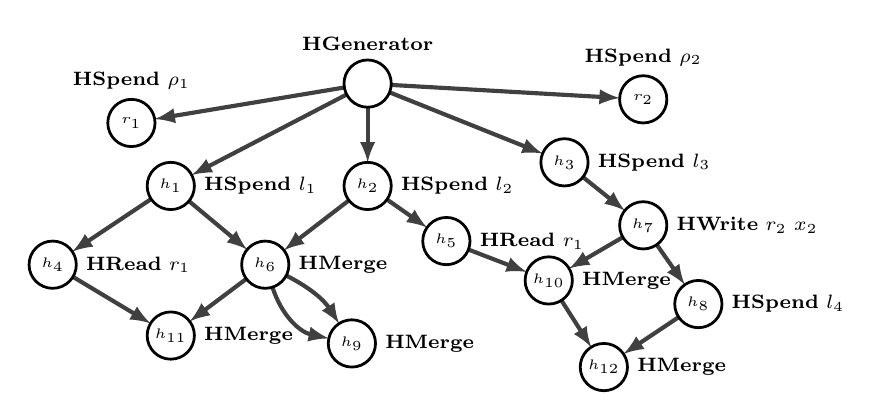
\begin{tikzpicture}
\SetVertexStyle[FillOpacity=0]
\Vertex[label=$\mathbf{HGenerator}$,x=0,y=0,position=above]{H0}
\Vertex[y=-1.3,x=-2.5,label=$\mathbf{HSpend}\ l_1$,position=0]{L1}
\Vertex[y=-1.3,x=0,label=$\mathbf{HSpend}\ l_2$,position=0]{L2}
\Vertex[y=-1,x=2.5,label=$\mathbf{HSpend}\ l_3$,position=0]{L3}
\Vertex[y=-2.3,x=-4,label=$\mathbf{HRead}\ r_1$,position=0]{R1}
\Vertex[y=-2,x=1,label=$\mathbf{HRead}\ r_1$,position=0]{R2}
\Vertex[y=-2.3,x=-1.3,label=$\mathbf{HMerge}$,position=0]{M1}
\Vertex[y=-1.8,x=3.5,label=$\mathbf{HWrite}\ r_2\ x_2$,position=0]{W1}
\Vertex[y=-2.8,x=4.2,label=$\mathbf{HSpend}\ l_4$,position=0]{S4}
\Vertex[y=-3.3,x=-0.2,label=$\mathbf{HMerge}$,position=0]{M2}
\Vertex[y=-3.6,x=3.0,label=$\mathbf{HMerge}$,position=0]{M3}
\Vertex[y=-3.2,x=-2.5,label=$\mathbf{HMerge}$,position=0]{M4}
\Vertex[y=-2.5,x=2.3,label=$\mathbf{HMerge}$,position=0]{M5}
\SetTextStyle[TextFont=\tiny]
\Text[y=-1.3,x=-2.5]{$h_1$}
\Text[y=-1.3,x=0]{$h_2$}
\Text[y=-1,x=2.5]{$h_3$}
\Text[y=-2.3,x=-4]{$h_4$}
\Text[y=-2,x=1]{$h_5$}
\Text[y=-2.3,x=-1.3]{$h_6$}
\Text[y=-1.8,x=3.5]{$h_7$}
\Text[y=-2.8,x=4.2]{$h_8$}
\Text[y=-3.3,x=-0.2]{$h_9$}
\Text[y=-3.6,x=3.0]{$h_{12}$}
\Text[y=-3.2,x=-2.5]{$h_{11}$}
\Text[y=-2.5,x=2.3]{$h_{10}$}
\Edge[Direct](H0)(L1) \Edge[Direct](H0)(L2) \Edge[Direct](H0)(L3)
\Edge[Direct](L1)(R1) \Edge[Direct](L1)(M1) \Edge[Direct](L2)(M1) \Edge[Direct](L3)(W1)
\Edge[Direct,bend=15](M1)(M2) \Edge[Direct,bend=-30](M1)(M2)
\Edge[Direct](W1)(S4) \Edge[Direct](R1)(M4) \Edge[Direct](M1)(M4) \Edge[Direct](S4)(M3)
\Edge[Direct](L2)(R2) \Edge[Direct](W1)(M5) \Edge[Direct](R2)(M5) \Edge[Direct](M5)(M3)

\Vertex[y=-0.5,x=-3.0,label=$\mathbf{HSpend}\ \rho_1$,position=above]{R1}
\Vertex[y=-0.2,x=3.5,label=$\mathbf{HSpend}\ \rho_2$,position=above]{R2}
\Text[y=-0.5,x=-3.0]{$r_1$}
\Text[y=-0.2,x=3.5]{$r_2$}
\Edge[Direct](H0)(R1) \Edge[Direct](H0)(R2)

\end{tikzpicture}
\caption{历史流的示例} \label{fig:His1}
\end{figure}

历史流表述了汇点的所有依赖对系统资源的访问历史,而系统资源的键 ResKey 是用历史流表示的。
首先历史流足以表达所有的系统资源键,实际上字符串就足以表达所有系统资源键的,
例如“文件:/某个/文件/的/路径”或者“内存:12345678地址”,所有字符串是无穷的而对一个程序
有意义的系统资源是有限的或同构于自然数集的无限,而字符串集同构于自然数集同构于历史流集。
另一方面系统资源可能随着程序的进行而产生,如动态分配的内存,用历史流表示资源键的好处是,
在某个历史点$h_1$表示的操作进行后若产生了一个新的系统资源(比如新分配了某段内存),
其键就可以表示为$\mathbf{HSpend}\ l\ h_1$
而与在别的历史点$h_2$上产生的资源$\mathbf{HSpend}\ l\ h_2$ 区分开来,
而资源键的标号可以简单地费用为0地表示 $l=\mathbf{Label}\ "resource\ name"\ 0$.
图\ref{fig:His1}中的 $r_1$ $r_2$ 是这样的例子。

其他一些特性也值得关注。如果两个历史流执行了完全相同的操作,那么这两个历史流是相等的。
而 $\mathbf{HSpend}$ 除了标记操作的费用还用以区分不同的操作。
例如图\ref{fig:His1}中,$h_4$与$h_5$的对$r_1$的读取发生在不同的操作$h_1$与$h_2$之后,
$h_1$与$h_2$使用不同的标号$l_1$与$l_2$区分开来,若$l_1=l_2$则$h_1=h_2$且$h_4=h_5$。
即两个线程若执行完全相同的操作则这两个线程的历史流亦是相同的,这导致在抽象机中
实际上无法区分开这两个线程。这是合理的并被认为是种优点,抽象机是基于数理逻辑的,
若两个线程执行了完全的操作则其运算的结果也是一样的

\section{用于本工作的抽象机的正式定义}


	
	\ZJUbackmatter
	%%%%%%%%%%%%%%%%%%%%%%%%%%%%%%
	%% 参考文献
	%%%%%%%%%%%%%%%%%%%%%%%%%%%%%%
	\ZJUthesisbib{bib}
	
	%%%%%%%%%%%%%%%%%%%%%%%%%%%%%%
	%% 发表论文目录
	%%%%%%%%%%%%%%%%%%%%%%%%%%%%%%
	\input{./chapters/publications}
	
	%%%%%%%%%%%%%%%%%%%%%%%%%%%%%%
	%% 致谢页
	%%%%%%%%%%%%%%%%%%%%%%%%%%%%%%
	\input{./chapters/thanks}
	
	
\end{document}
